\chapter{NodeGit}

NodeGit\footnote{\url{http://www.nodegit.org/}} je knihovna pro programovací jazyk JavaScript se záměrem zpřístupnit základní funkce Gitu implementované projektem libgit2\footnote{\url{https://libgit2.github.com/}} v jazyce C. Libgit2 se hojně využívá pro široké spektrum i jiných programovacích jazyků, například pro jazyk Ruby na něm staví Rugged\footnote{\url{https://github.com/libgit2/rugged}}, pro .NET LibGit2Sharp\footnote{\url{https://github.com/libgit2/libgit2sharp}}, Python pygit2\footnote{\url{http://www.pygit2.org/}}, PHP php-git\footnote{\url{https://github.com/libgit2/php-git}} a spoustu dalších\footnote{\url{https://github.com/libgit2/libgit2\#language-bindings}}. Vážnost projektu nepředstavují jen knihovny všemožných jazyků, ale i velké firmy, které na tuto implementaci spoléhají; jedná se například o Microsoft, Bitbucket, Canonical \cite{libgit2-companies}. Konkrétně u JavaScriptové nadstavby pak GitKraken či GitHub \cite{nodegit-products}. Nehledě na velkou rozšířenost, libgit2 a v souvislosti s ním i NodeGit osahují jisté neduhy, které byly objeveny při vývoji Aplikace a vzhledem k tomu, že měly velký vliv, bude se jim tato kapitola věnovat. Některé jsou již nahlášené v~příslušných repozitářích jako bug, ostatní jsou specifické pro tuto bakalářskou práci.

\section{Webpack}

% @TODO: https://webpack.github.io/ http://gulpjs.com/ https://gruntjs.com/ https://facebook.github.io/react/ https://facebook.github.io/react/docs/introducing-jsx.html
Pro větší projekty psané v JavaScriptu je běžné využití některého z nástrojů pro správu kódu, jeho strukturu, rozšíření. Typickými zástupci jsou Gulp, Grunt a Webpack. Vzhledem k velké popularitě a podpoře Reactu byla Aplikace vyvýjena pomocí Webpacku, což umožňovalo například zjednodušenou syntaxy JSX, která významně zpřehledňuje zápisy šablon pro React, jež se více podobají zápisu v HTML.

\begin{listing}[ht]
\begin{minted}[]{javascript}
e(
	Card,
	{
		key: i,
		style,
	},
	e(
		CardTitle,
		{
			title: project.name,
			subtitle: project.note,
			style: {
				cursor: 'pointer',
			},
			onTouchTap: () => this.selectProject(project),
		}
	)
)
\end{minted}
\caption[Komponenta v JavaScriptu]{Zápis pro vykreslení komponenty Reactu v běžném JavaScriptu}
\end{listing}

\begin{listing}[ht]
\begin{minted}[]{javascript}
<Card key={i} style={style}>
	<CardTitle
		title={project.name}
		subtitle={project.note}
		style={{ cursor: 'pointer' }}
		onTouchTap={() => this.selectProject(project)}
	/>
</Card>
\end{minted}
\caption[Komponenta v JSX]{Zápis pro vykreslení stejné komponenty Reactu v JSX}
\end{listing}

\begin{listing}[ht]
	\begin{minted}[]{javascript}
const Card = require('material-ui/Card').Card
const CardTitle = require('material-ui/Card').CardTitle
	\end{minted}
	\caption[Závislosti v JavaScriptu]{Závislost na Card a CardTitle v běžném JavaScriptu}
\end{listing}

\begin{listing}[ht]
	\begin{minted}[]{javascript}
import { Card, CardTitle } from 'material-ui/Card'
	\end{minted}
	\caption[Závislost v JSX]{Závislost na Card a CardTitle v JSX}
\end{listing}

\FloatBarrier

Předchozí čtyři ukázky znázorňují výhody JSX ve stručnosti a přehlednosti díky upravenému zápisu komponent a modernější sytaxy \uv{import from}. Mimo to umí Webpack například i rozpoznávání využitých závislostí a na základě toho tvořit menší produkční sestavení aplikací. Z těchto zlepšení bylo zhruba po dobu poloviny vývoje těženo, ale ukázalo se, že Webpack bez upozornění ubírá z knihovny NodeGit některé funcionality, jež se začínaly stávat kritickými. Po mnoha neúspěšných pokusech změny konfigurace Webpacku, aby spávně pracoval s knihovnou, která je závislá na binárním kódu libgit2, byl Webpack z projektu odebrán a stávající kód přepsán do běžného JavaScriptu. Přesná příčina komplikací nebyla doposud objevena vzhledem k unikátní kombinaci NodeGitu a Webpacku.

\section{Git clone}

Další problematickou fází vývoje byla práce s metodou pro klonování repozitářů, které se týkají dva problémy.

\subsection{Nekonečné trvání}

Metodu pro klonování repozitářů, s funkcionalitou podle dokumentace\footnote{\url{http://www.nodegit.org/api/clone/}} srovnatelnou s \mintinline{bash}{git clone repository}, nebylo možné použít, protože ve chvíli, kdy například volání mělo selhat z důvodu špatných přístupových údajů uživatele, metoda implementovaná jako JavaScriptová \uv{Promise} nikdy neskončila úspěchem ani neúspěchem, což znemožnilo možnost informovat uživatele o výsledku a patřičně aktualizovat uživatelské rozhraní. Náhradním řešením bylo ustoupení od metody Clone nahrazením za sérii jiných. Nyní se namísto klonování nejdříve lokálně inicializuje prázdný repozitář, do kterého se poté přidá URL repozitáře jako remote origin a následně spustí fetch na tento origin. Pokud již repozitář něco obsahuje na hlavní větvi, provede se provázání s~větví lokální, tj. vytvoření lokální větve a nastavení upstreamu.

\subsection{Chyba nevracející řízení}

Náhradní řešení je však nestabilní. Během několikaměsíční intenzivní práce s NodeGitem se jednou vyvovala chybová hláška Microsoft Visual C++ Runtime Library v prostředí Windows, která nebyla správně zachycena a zpracována standardně implementací libgit2 či nadstavbou NodeGitu. Narozdíl od metody pro klonování tato chyba byla zobrazena po manipulaci s větvemi při vytváření lokální pro spárování se vzdálenou. Chybu nebylo možné opakovaně vyvolat stejným kódem Aplikace, takže nešlo rozumně vymyslet nové náhradní řešení. Vzhledem k unikátnosti je tento stav považován za velice nepravděpodobný, avšak v dalším vývoji je nutno dbát ohled na toto nebezpečí vzhledem k~tomu, že se opět jedná o Promise, JavaScriptový příslib, který nemusí být nikdy naplněn ani zamítnut. Tím pádem v takové chvíli nemůže stejně jako v předchozím bodě být aktualizováno uživatelské rozhraní či zopakovaní poslední neúspěšné akce a navíc uživatel je zatížen hláškou v angličtině, která pro něho nemusí být nikterak vypovídající. Vzhledem k nemožnosti reprodukce je následující obrázek pouze v původním základním rozlišení.

\FloatBarrier
\begin{figure}[h]
	\centering
	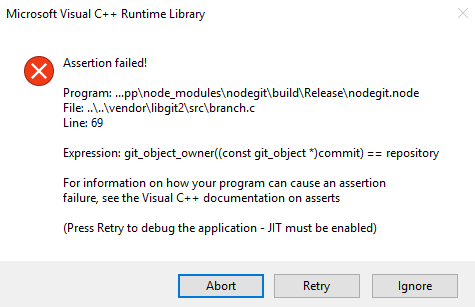
\includegraphics[width=\textwidth]{sections/nodegit/images/branch.png}
	\caption{Chybová hláška}
\end{figure}
\FloatBarrier

\section{Git status}

Na obrazovce uživatelského rozhraní Aplikace pro vytvoření nového commitu se mohou zobrazovat tři různé druhy souborů. Změněné soubory jsou buď připravené pro commit, nebo nejsou a v repozitáři jsou známé či neznámé.

\subsection{Odebrání smazaného souboru}

NodeGit poskytuje pro přidávání do a odebírání z připravených položek (staging area) dvě metody, \mintinline{javascript}{Index.add(path)}\footnote{\url{http://www.nodegit.org/api/index/\#add}} a \mintinline{javascript}{Index.remove(path)}\footnote{\url{http://www.nodegit.org/api/index/\#remove}}. Obě metody přijímají jako argument cestu, řetězec znaků, které určují polohu souboru v lokálním souborovém systému. V obou případech dochází k chybě při manipulaci se souborem, který se v systému již nenachází. Pomocí těchto metod tedy nejde pracovat s přidávání a odebíráním neexistujících souborů na a ze stage. Alternativu NodeGit nenábízí. Řešením je tedy systémové volání v~JavaScriptu, které umožňuje přístup k příkazovému řádku, na kterém lze spouště příkazy \mintinline{bash}{git}. Pro fungování tohoto postupu je nutná instalace programu git a přidání do systémové cesty pro spustitelné programy na zařízení uživatele.

\FloatBarrier
\begin{listing}[ht]
	\begin{minted}[]{javascript}
const exec = require('child-process-promise').exec
exec(`cd ${projectPath} && git add "${filePath}"`))
	\end{minted}
	\caption{Přidání smazaného souboru}
\end{listing}
\FloatBarrier

\subsection{Výpis neznámých souborů}

Se smazanými soubory má problémy i metoda na zjištění změněných souborů \mintinline{javascript}{Repository.getStatus()}\footnote{\url{http://www.nodegit.org/api/repository/}}. Pro smazané, případně přejmenované, soubory vrací neúplná data, se kterými není možné dále pracovat. Stejně jako v předchozím bodě, dokumentace a ukázky\footnote{\url{https://github.com/nodegit/nodegit/tree/master/examples}} NodeGitu nepočítají s odstraněnými soubory. V tomto případě je však mezi uživateli známo náhradní řešení, které pomocí metody \mintinline{javascript}{Diff.indexToWorkdir(...)} vyhledá všechny změněné neignorované soubory či adresáře a vrátí jejich cesty, se kterými lze dále snadno pracovat pomocí systémových volání \mintinline{bash}{git add path} či \mintinline{bash}{git reset HEAD path}.

\section{Konflikty}

Během slučování stavu na vzdáleném serveru a stavu v lokálním repozitáři může dojít ke kolizím v případě, že například oba stavy obsahují v historii nové změny stejného souboru na stejných řádcích. V takovém případě je nutno rozhodnout, které změny zůstanou po sloučení, případně typicky uživatel má možnost ručně udělat změny nové, které berou oba zdroje v potaz. Aplikace automaticky preferuje změny ze vzdáleného repozitáře, což je omezení nedokonalosti metod NodeGitu pro slučování, které může vést ke nezpozorované ztrátě změn či k nevalidnímu kódu projektu. V historii vše zůstává zazálohované. Aplikace na toto nebezpečí upozorňuje po sloučení zprávou ve Snackbaru. NodeGit při výskytu kolize udržuje stav souborů pouze v paměti, což omezuje uživatelovi možnosti, jak nesrovnalosti napravit. Pravděpodobně nejlepším řešením by bylo promítnout soubory do souborového systému, aby je uživatel mohl upravit ve vlastním editoru, jako se to běžné dělá při klasickém používání příkazu \mintinline{bash}{git merge} či \mintinline{bash}{git pull}.

\section{Autentizace}

Velice problematické bylo ověřování uživatele na vzdálených serverech z několika důvodů, rozebraných v následujících podkapitolách.

\subsection{Vzdálené servery}

GitHub, Bitbucket i GitLab mají odlišné odpovědi v případě, že se k nim snaží připojit někdo s navalidními přihlašovacími údaji. Vzhledem k tomu, že knihovna NodeGit poskytuje přístup pouze k textové podobně těchto odpovědí, je složité na ně programově reagovat. Kvůli tomu, že jsou v angličtině a nejsou typicky určené pro nezkušené uživatele, není možné je jen zobrazit a nechat jejich řešení na uživateli.

Zatím byly vypozorovány tyto situaci, při kterých dochází k zamítnutí:

\begin{itemize}
	\item uživatel poskytl špatné přihlašovací údaje,
	\item uživatel nemá správně nastaveného agenta pro správu SSH klíčů (na Windows Pageant),
	\item uživateli nebyl nikým udělen přístup do repozitáře,
	\item uživatel byl zablokován kvůli několika nezdařeným pokusů o autentizaci (tento stav byl odhalen u~Bitbucketu, který pro odblokování vyžaduje přihlášení přes webové rozhraní, podobně blokuje i GitLab).
\end{itemize}

\subsection{Uložiště přístupových údajů}

Pro ukládání přístupových údajů pro HTTPS spojení využívá Aplikace standardní funkce Gitu, Credential Store\footnote{\url{https://git-scm.com/docs/git-credential-store}}. Tato funkce však nezaručuje, že údaje poskytne vždy a že jejich změnu si zapamatuje. Není tedy vhodné se na ni spoléhat. Jako dočasné řešení je přimět uživatele spustit příkaz pro nastavení trvalého ukládání přihlašovacích údajů na disk.

\FloatBarrier
\begin{listing}[ht]
	\begin{minted}[]{bash}
git config --global credential.helper store
	\end{minted}
	\caption{Nastavení ukládání přístupových údajů na disk}
\end{listing}
\FloatBarrier

\subsection{Správce klíčů pro SSH}

NodeGit nepodporuje správce klíčů OpenSSH\footnote{\url{https://www.openssh.com/}} na Windows. Je tedy nutné doinstalovat alternativu Pageant. Navíc je o neběžícím agentu uživatele složité informovat, protože NodeGit tento stav nerozlišuje a poskytuje stejná data i v případě, že Pageant běží, ale pro konkrétní server neposkytuje klíče.

\subsection{cURL}

Během vývoje došlo k několika chybám na linuxové platformě týkající se chyby libcurl\footnote{\url{https://curl.haxx.se/libcurl/}}. Zatím se problém neopakuje. Každopádně závislost NodeGitu na správné konfiguraci platformy je kritická a nevylučuje se, že podobné selhání mohou nastat znovu.

\section{Řešení}

Zmíněné problémy výrazně ovlivňují stabilitu Aplikace, její funkcionality a možnost dalšího rozvoje. Je vhodné zvážit, jestli závislost na NodeGitu odstranit a nahradit třeba systémovým volání příkazu \mintinline{bash}{git --porcelain}, jenž poskytuje strojově čitelné odpovědi na všechny potřebné operace.
